\documentclass[]{report}
\usepackage{titlesec}
\usepackage{graphicx}

\usepackage[sfdefault]{roboto}

%PdfTeX settings for a correct UTF 8 Mapping
%------------------------------------------------------
\usepackage{ifpdf}
\ifpdf    \input{glyphtounicode.tex}    %Part of modern distribution
%%%\input{glyphtounicode-cmr.tex}     %Additionnal glyph: You must grab it from pdfx package
\pdfgentounicode=1
\else  %Place here the settings for other compilator
\fi


%Encoding + cmap (to get proper UTF8 mapping)
%------------------------------------------------------
\usepackage{cmap}
\usepackage[utf8]{inputenc}
\usepackage[T1]{fontenc}
 
\usepackage{listings}



\titleformat{\chapter}{\normalfont\huge}{\thechapter.}{20pt}{\huge\textbf}

\usepackage{color}   %May be necessary if you want to color links
\usepackage{hyperref}
\hypersetup{
	colorlinks=true, %set true if you want colored links
	linktoc=all,     %set to all if you want both sections and subsections linked
	linkcolor=black,  %choose some color if you want links to stand out
}

% Title Page
\title{PJP Seminarski\\Kompajler za programski jezik B}
\author{Adnan Elezović (16728)}


\begin{document}
	
	\maketitle
	
	\renewcommand{\contentsname}{Sadržaj}
	
	\chapter{Uvod}
	Ovaj rad se fokusirao na implementaciju kompajlera za programski jezik B. Za početak razvoja uzet je B.ATG fajl koji se koristio za vježbe i implementirane su sve preostale funkcionalnosti.
	
	\section{Radno okruženje}
	Da bi se priloženi kompajler mogao koristiti, priložene su pomoćni fajlovi za jednostavno testiranje. 
	Ovo uključuje build skriptu, kao i \textbf{.OBJ} fajlove sa nekim built in funkcijama ( \textbf{scanf, printf, getchar, putchar i fputs}). 
	Priloženi fajlovi su kompajlirani za x86 arhitekturu pa zahtjevaju odgovarajuće radno okruženje.
	Startup rutinu indirektno pozivamo kroz kratki pomoćni program \textbf{driver.c}. On se statički linkuje sa izlazom našeg B kompajlera i poziva predefiniranu proceduru koja nam predstavlja početak B programa. Ispod je data slika koja prikazuje opisani proces.
	\begin{center}
		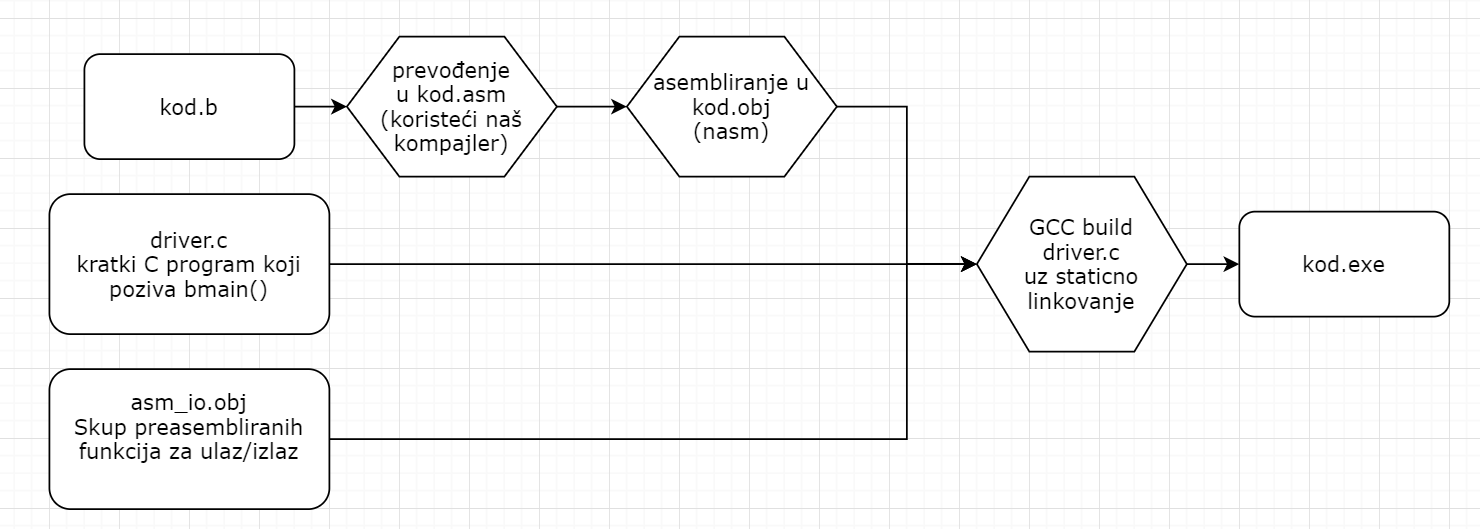
\includegraphics[scale=0.5]{diag1.png}
	\end{center}
	
	\chapter{Tipovi podataka}
	Podržani su cjelobrojni tipovi podataka, kao i nizovi čiji su elementi cjelobrojnog tipa. Pored ovoga omogućen je ograničen rad sa stringovima. Pošto B ne podržava adresiranje bajtova, manipulacija stringova je jako nepraktična.
\end{document}

